\documentclass{beamer}

\input{../../spec_files/course_preamble.tex}
\subtitle{Foundations of Neuro-Symbolic AI}
\date{Summer Term 2026}
\author[FONS]{Alex Goessmann}
\institute[]{
    University of Applied Science Würzburg-Schweinfurt
%    Weierstrass Institute for Applied Analysis and Stochastic
}

%\newcommand{\techwstitle}{
%\small
%%Workshop \\
%Logik für Erklärbare KI:
%Technische Einführung in das ENEXA Projekt}
%\newcommand{\smalltechwstitle}{ENEXA Workshop}

%\newcommand{\techwsdate}{15.+16. July, 2024}

%\newcommand{\techwsauthors}{
%Alex Goessmann
%}

%\newcommand{\techwsinclude}{
%	\usepackage{../../spec/beamercolorthemeclaw}
%	\usepackage{/Users/alexgoessmann/Documents/ENEXA/latex_macros/beamer_template/beamerfontthemeclaw}
%	\usepackage{/Users/alexgoessmann/Documents/ENEXA/latex_macros/beamer_template/beamerinnerthemeclaw}
%	\usepackage{/Users/alexgoessmann/Documents/ENEXA/latex_macros/beamer_template/beamerouterthemeclaw}
%
%	\input{/Users/alexgoessmann/Documents/ENEXA/latex_macros/packages.tex}
%	\input{/Users/alexgoessmann/Documents/ENEXA/latex_macros/macros.tex}
%	\input{/Users/alexgoessmann/Documents/ENEXA/latex_macros/macros_tc.tex}
%	\input{/Users/alexgoessmann/Documents/ENEXA/latex_macros/tikz_blocks.tex}
%
%	\subtitle{\techwstitle}
%	\date[\techwsdate]{\techwsdate}
%	\author[\smalltechwstitle]{\techwsauthors}
%	\institute[]{\eupic}
%}

\newcommand{\techwschapterone}{I-Tensors}
\newcommand{\techwschaptertwo}{II-Probabilities}
\newcommand{\techwschapterthree}{III-Logics}
\newcommand{\techwschapterfour}{IV-Applications}

\newcommand{\eupic}{
\begin{center}
	%\includegraphics[width=4cm]{/Users/alexgoessmann/Documents/ENEXA/latex_macros/images/fundedEU.png}
\end{center}
}

\newcommand{\enexadateveublock}{
\begin{center}\begin{tikzpicture}
  	%\node [anchor=center] at (0,0) {\includegraphics[width = 1.5cm]{/Users/alexgoessmann/Documents/ENEXA/latex_macros/images/DATEV.png}};
	%\node [anchor=center] at (2.5,0.5) {\includegraphics[width = 3.5cm]{/Users/alexgoessmann/Documents/ENEXA/latex_macros/images/enexa.png}};
	%\node [anchor=center] at (2.55,-0.5) {\includegraphics[width = 3cm]{/Users/alexgoessmann/Documents/ENEXA/latex_macros/images/fundedEU.png}};
\end{tikzpicture}\end{center}
}


%% OLD
\newcommand{\aselectionvariable}{L}
\newcommand{\vselectionvariable}{L}
\newcommand{\fselectionvariable}{L}
\newcommand{\cselectionvariable}{L}
\newcommand{\individualorder}{n}
\newcommand{\variableof}[1]{\indvariableof{#1}}
\newcommand{\sindex}{s}
\newcommand{\pindex}{p}
\newcommand{\oindex}{o}
\newcommand{\exquery}{q}
%\newcommand{\datapointof}[1]{x^{#1}}
\newcommand{\atomicqueryof}[1]{g_{#1}}
\newcommand{\facsystem}{\shortcatvariables}
\newcommand{\margprobof}[1]{\probat{#1}}
\newcommand{\mlnprobabilityof}[1]{\expdistof{#1}}
%\newcommand{\oldenexadateveublock}{
%	\begin{center}
%	\begin{minipage}{0.2\textwidth}
%		\begin{center}
%			\includegraphics[width = 2.5cm]{images/DATEV.png}
%		\end{center}
%	\end{minipage}
%	\begin{minipage}{0.55\textwidth}
%		\begin{center}
%			\includegraphics[width=5.5cm]{images/enexa.png} \\
%			\includegraphics[width=5.5cm]{images/fundedEU.png} \\
%		\end{center}
%	\end{minipage}
%	\end{center}
%}

\title[Empirical Distributions]{
	\techwschaptertwo \\
	{\huge Empirical Distributions: Representation of Samples}
}

\begin{document}

{\frame[plain]{\titlepage}}



%
%\begin{frame}{Observations of a Factored System}
%
%\begin{example}[Students and their semester]
%	We ask (pairs of) students about their semester and want to capture the statistics.
%\end{example}
%
%\begin{block}{Task: Representation of Observations}
%	Let there be observations of the system by a set of states
%		\[ \{(\catindicesof{\datindex}) \, : \, \datindexin \} \, . \]
%	How to capture them by tensors?
%\end{block}
%
%Aim: 
%\begin{itemize}
%	\item Represent the observations for querying
%	\item Find models making sense out of the observations
%\end{itemize}
%
%\end{frame}
%
%
%\begin{frame}{Formalization with a sample selector map}
%
%Given a dataset $\{(\catindicesof{\datindex}) \, : \, \datindexin \}$ of samples of the factored system we define the sample selector map
%	\[ \datamap : [\datanum] \rightarrow \facstates \]
%
%\medskip
%
%\begin{block}{Idea}
%	Enrich the factored system with variables $\catvariables$ by a data selection variable $\datvariable$ and encode $\datacore$ using the one-hot encoding of the larger system.
%\end{block}
%
%
%\end{frame}



\section{Empirical Distributions}


\begin{frame}{Observations of a Factored System}

\begin{example}[Students and their semester]
	We ask students about their semester and want to capture the statistics.
\end{example}

\begin{block}{Task: Representation of Observations}
	Let there be observations of the system by a set of states
		\[ \{(\catindicesof{\datindex}) \, : \, \datindexin \} \, . \]
	How to capture them by tensors?
\end{block}

Aim: 
\begin{itemize}
	\item Represent the observations for querying
	\item Find models making sense out of the observations
\end{itemize}

\end{frame}


\begin{frame}{Formalization with a sample selector map}

Given a dataset $\{(\catindicesof{\datindex}) \, : \, \datindexin \}$ of samples of the factored system we define the sample selector map
	\[ \datacore : [\datanum] \rightarrow \facstates \]

\medskip

\begin{block}{Idea}
	Enrich the factored system with variables $\catvariables$ by a data selection variable $\aselectionvariable$ and encode $\datacore$ using the one-hot encoding of the larger system.
\end{block}


\end{frame}


\begin{frame}{More general: Encoding of maps between Factored Systems}

\begin{definition}
	Let $\exfunction$ be a function
		\[ \exfunction : \facstates \rightarrow  \secfacstates \]
	which maps the states of a factored system to variables $\catvariables$ to the states of another factored system with variables $\seccatvariables$.
	Then the tensor representation of $\exfunction$ is a tensor
		\[ \bencodingof{\exformula} \in \left(\exfunctiontargetspace\right)  \otimes \left(\facspace\right) \]
	defined by
		\[ \bencodingof{\exformula} = \sum_{\catindexofin{0}} \cdots  \sum_{\catindexofin{\atomenumerator-1}}  \onehotmapof{\exfunction(\catindices)} \otimes \onehotmapof{\catindices} \, . \]
\end{definition}

\end{frame}



\begin{frame}{Data tensor}

In the case of the sample selection map
	\[ \datamap : [\datanum] \rightarrow \facstates \]
we have a representation tensor called the \emph{data tensor}
	\[ \datacore = \sum_{\datindexin} \onehotmapof{\datindex} \otimes \onehotmapof{\catindicesof{\datindex}} \,  \]
depicted as 
\begin{center}
	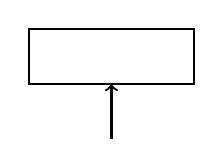
\begin{tikzpicture}[scale=0.35, thick] % , baseline = -3.5pt

\drawatomindices{0}{2}
\draw (-1,1) rectangle (5,-1);
\node[anchor=center] (text) at (2,0) {$\datacore$};
\draw[<-] (2,-1) -- (2,-3) node[midway, right] {\tiny $\datvariable$};


\end{tikzpicture}
\end{center}

\begin{block}{Representation of Data}
	The one-hot encoding of each observation is stored on a slice of the data tensor.
\end{block}

\end{frame}


%\begin{frame}{}
%\end{frame}


\begin{frame}{Average of the Observation}

The \emph{empirical distribution} is the average of the one-hot encoded observed states:
\begin{align*}
	\empdistribution \coloneqq \frac{1}{\datanum}\sum_{\datindexin} \onehotmapof{\catindicesof{\datindex}}
\end{align*}

In a contraction diagram we denote the average by % Already the decomposition!
\begin{center}
	\begin{tikzpicture}[scale=0.35, thick] % , baseline = -3.5pt


    \drawatomindices{0}{2}
    \draw (-1,1) rectangle (5,-1);
    \node[anchor=center] (text) at (2,0) {$\empdistribution$};


    \node[anchor=center] (text) at (7,0) {${=}$};

    \node[anchor=center] (text) at (22,-1) {${\cdot}$};

    \begin{scope}
        [shift={(10,2)}]

        \newcommand{\conposseldec}{4.5,-5.5}

        \draw[fill] (\conposseldec) circle (\dotsize);
        \draw[-<-] (\conposseldec) -- (4.5,-7.5) node[midway, right] {\colorlabelsize $\datvariable$};
        \draw (3.5,-7.5) rectangle (5.5, -9.5);
        \node[anchor=center] (text) at (4.5,-8.5) {\corelabelsize $\frac{1}{\datanum} \ones$};

        \draw[-<-] (0,1) -- (0,-1) node[midway,left] {\colorlabelsize $\catvariableof{0}$};
        \draw (-1,-1) rectangle (1, -3);
        \node[anchor=center] (text) at (0,-2) {\corelabelsize $\datacoreof{0}$};
        \draw[-<-] (0,-3) to[bend right=20] (\conposseldec);


        \draw[-<-] (3,1) -- (3,-1) node[midway,left] {\colorlabelsize $\catvariableof{1}$};
        \draw (2,-1) rectangle (4, -3);
        \node[anchor=center] (text) at (3,-2) {\corelabelsize $\datacoreof{1}$};
        \draw[-<-] (3,-3) to[bend right=20]  (\conposseldec);

        \node[anchor=center] (text) at (6,-2) {$\cdots$};

        \draw[-<-] (9,1) -- (9,-1) node[midway,left] {\colorlabelsize $\catvariableof{\atomorder-1}$};
        \draw (7.75,-1) rectangle (10.25, -3);
        \node[anchor=center] (text) at (9,-2) {\corelabelsize $\datacoreof{\atomorder-1}$};
        \draw[-<-] (9,-3) to[bend left=20]  (\conposseldec);


    \end{scope}


\end{tikzpicture}
\end{center}

\end{frame}


\begin{frame}{More efficient data representation}

The storage demand of $\datacore$ \emph{increases exponentially }
	\[ \mathrm{dim}\left[\datacore\right] = \left( \facdim \right) \cdot \datanum \, . \]

\begin{block}{Store the values $\catvariableof{\atomenumerator}$ separately for each $\atomenumeratorin$!}

\medskip

The collection of encoding tensors
	\[ \datacoreof{\atomenumerator} \in \rr^{\catdimof{\atomenumerator}\times\datanum} \]
to the maps
	\[ \datamap_{\atomenumerator} :[\datanum] \rightarrow [\catdimof{\atomenumerator}] \quad , \quad  \datamap_{\atomenumerator}(\datindex) =  \catindex^{\datindex}_{\atomenumerator}\]
%defined by
%	\[ \datacoreof{\atomenumerator}_{: \datindex} =\onehotmapof{\catindexof{\atomenumerator}^\datindex} \]
has a \emph{linearly increasing} storage demand of 
	\[ \sum_{\atomenumeratorin} \mathrm{dim}\left[\datacoreof{\atomenumerator}\right] = \sum_{\atomenumeratorin} \catdimof{\atomenumerator}\cdot \datanum \, .  \]

\end{block}
\end{frame}


\begin{frame}{Representation of the Empirical in a CP Format}

The data tensor can be stored by the contraction
	\[ \contractionof{\bencodingof{\datamap}}{\catvariableof{0},\ldots,\catvariableof{\atomenumerator-1},\datvariable} =
	\contractionof{\datacoreof{0},\ldots,\datacoreof{\atomorder-1}}{\catvariableof{0},\ldots,\catvariableof{\atomorder-1},\datvariable} \]
depicted as
\begin{center}
	\begin{tikzpicture}[scale=0.35, thick] % , baseline = -3.5pt





\drawatomindices{0}{2}
\draw (-1,1) rectangle (5,-1);
\node[anchor=center] (text) at (2,0) {$\datacore$};
\draw[<-] (2,-1) -- (2,-3) node[midway, right] {\tiny $\datvariable$};

\node[anchor=center] (text) at (7,0) {${=}$};


\begin{scope}[shift={(10,2)}]

\newcommand{\conposseldec}{4.5,-5.5}

\draw[fill] (\conposseldec) circle (0.25cm);
\draw[<-] (\conposseldec) -- (4.5,-7.5) node[midway, right] {\tiny $\datvariable$};
%\draw[dashed] (3.5,-7.5) rectangle (5.5, -9.5);
%\node[anchor=center] (text) at (4.5,-8.5) {\small $\frac{1}{\datanum} \ones$};

\draw[<-] (0,1) -- (0,-1) node[midway,left] {\tiny $\catvariableof{0}$};
\draw (-1,-1) rectangle (1, -3);
\node[anchor=center] (text) at (0,-2) {\small $\datacoreof{0}$};
\draw[<-] (0,-3) to[bend right=20] (\conposseldec);


\draw[<-] (3,1) -- (3,-1) node[midway,left] {\tiny $\catvariableof{1}$};
\draw (2,-1) rectangle (4, -3);
\node[anchor=center] (text) at (3,-2) {\small $\datacoreof{1}$};
\draw[<-] (3,-3) to[bend right=20]  (\conposseldec);

\node[anchor=center] (text) at (6,-2) {$\cdots$};

\draw[<-] (9,1) -- (9,-1) node[midway,left] {\tiny $\catvariableof{\atomorder-1}$};
\draw (8,-1) rectangle (10, -3);
\node[anchor=center] (text) at (9,-2) {\small $\datacoreof{\atomorder-1}$};
\draw[<-] (9,-3) to[bend left=20]  (\conposseldec);




\end{scope}

		


\end{tikzpicture}
\end{center}
This is called a \emph{CP Tensor Decomposition}.

\begin{block}{CP Decomposition of Empirical Distributions}
	Instead of storing the datacore $\datacore$, store the encodings $\datacoreof{\atomenumerator}$.
\end{block}

\end{frame}



\end{document}